% TODO
% 
% 
% 
% 
% 
% 
\documentclass{article}
\usepackage{algorithm}
\usepackage{algpseudocode}
\usepackage{geometry}
\usepackage{xcolor}
\usepackage{graphicx}
\usepackage{mathtools}
\usepackage{enumitem}
\usepackage{amsmath,amsthm}
\usepackage[english]{babel}
\usepackage{amsfonts}
\usepackage{thmtools}
\usepackage{fancyhdr}
\graphicspath{{./IMG/}}
\usepackage{color}   %May be necessary if you want to color links
\usepackage{hyperref}
\hypersetup{
    colorlinks=true, %set true if you want colored links
    linktoc=all,     %set to all if you want both sections and subsections linked
    linkcolor=blue,  %choose some color if you want links to stand out
}

%-------------- HEADER -- FOOTER --------------------------------------------------------
% Main Title
\newcommand{\PaperTitle}{MAIN TITLE HERE}
% Sub Title
\newcommand{\PaperSubTitle}{SUBTITLE HERE}
% Authors
\newcommand{\Authors}{Aiden Taylor and Noah Pinel}

% Title Page
\title{
    % \vspace{2in}
    \textmd{\textbf{\PaperTitle\\ \PaperSubTitle}}\\
    \author{Created by \Authors}
    \date{}
    \vspace{6in}
}

%--- LAZY -----------------------------------------------------------------------------------
\newcommand{\R}{\mathbb{R}}
\newcommand{\Z}{\mathbb{Z}}
\newcommand{\ps}{\{p_n\}}



%---------------------HEADER FOOTER-----------------------------------------------------------
\pagestyle{fancy}
\fancyhead{}

\fancyhead[L]{\slshape\nouppercase{\leftmark}}
\rhead{MATH 327 Paper}
\fancyfoot{}
 
% Hide section for format purposes i.e ToC and Abstract.
\newcommand\invisiblesection[1]{%
  \refstepcounter{section}%
  \addcontentsline{toc}{section}{\protect\numberline{\thesection}#1}%
  \sectionmark{#1}}

%----------------START-------------------------------------
\begin{document}
\maketitle % Print the title
\thispagestyle{empty}
\newpage
\fancyfoot[R]{\thepage}
%----------------TABLE OF CONTENTS------------------------------------------
\tableofcontents
\invisiblesection{Table of contents}
\newpage
%----------------ABSTRACT---------------------------------------------------
\invisiblesection{Abstract}
\begin{abstract}
 Give a general Overview of our project, explain high level what we each did...
\end{abstract}
\newpage

% -------- NOAH WU #1/2 --------
\section{Implementation of The Sieve of Eratosthenes in Python}
\subsection{Overview}
The Sieve of Eratosthenes is a type of prime sieve. Prime sieves are algorithms 
that are very good at generating prime numbers up to some upper bound n, where $n\in\Z^+$.
The following sections explain the Implementation process of simulating the Sieve of Eratosthenes 
in the programming language Python.

\subsection{The Implementation}
My first run in with the sieve of Eratosthenes was during my number theory course, the 
mechanical nature of the sieve seemed to be a perfect way to utilize a computer to do
some interesting math. The entirety of the program relies on the algorithm below, so here 
are the meat and potatoes of the whole thing,
\begin{algorithm}
  \caption{: An algorithm for The Sieve of Eratosthenes}
  \begin{algorithmic}[1]
  \Require: $n > 0$
  \Ensure: List of prime numbers 2, ..., n
  \State Sieve$(n):$
      \State Populate a boolean list P size 2, ..., n.
      \State Initialize all index values to True.
      \For{$i = 2,..., n+1$:} 
          \State if P[i] TRUE
          \For{$j = i^2, i^2+1, i^2+3,..., n$:}
            \State set P$[j]$ False
          \EndFor
      \EndFor
    \State Return P
  \end{algorithmic}
\end{algorithm}\\
Simply put, we have a list of size $2,..., n$. We set all values of our list to True, then starting at 2 we loop through each index
setting multiples of the respected current position to false. After this has run, we are left with a list where all prime values are
unchecked, that is, they remain True while composite numbers are false. Below is a visual of the algorithm working for a list of size 10.
\begin{center}
  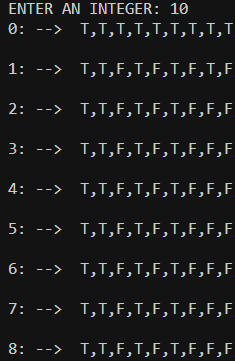
\includegraphics[scale=0.4]{Sieveiter.png}
\end{center}
We can see that after 8 iterations of following the algorithm the only index values set True are $2,3,5,7$, i.e., the first 4 primes. 
Now as cool as it is to visualize the algorithm I feel like finding the number of primes $\leq$ some large n is a lot more interesting.
To help with run time I disabled the visual aspect of the algorithm and was able to find a value for the primes up to $100,000,000$.
\begin{center}
  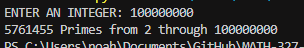
\includegraphics[scale=1.0]{primesFound.png}
\end{center}
Using the forbidden site Wolfram Alpha to verify, there are indeed 5,761,455 primes in between 2 and 100,000,000.
\subsection{Conclusion}
The last calculation presented took just about an epsilon under a minute to calculate, which for an algorithm that has been around for thousands of years
I feel is very impressive, thus, Eratosthenes sieve is a powerful tool to find primes up to some appropriate positive integer. This problem also displays the interplay between Mathematics 
and Computer Science and how they complement each other very well. The source code for Sieve.py will be included in our submission with documentation if you're
wanting to poke around.

\newpage
% -------- NOAH WU #1/2 --------
\section{Visual Representation of Euler's Phi Function}
\subsection{Overview}
Euler is one of the most well known Mathematicians ever, the following program I implemented 
is a visual representation of function he created, namely the Euler Phi function.
\subsection{What is it?}
Euler's Phi function takes in a positive value n, and counts the number of relatively prime numbers up to the original n.
For example $\Phi(10)= |\{1,3,7,9\}| = 4$, so Euler's function is telling us that from 1-10, there are 4 numbers coprime to 10.

\subsection{The Implementation}
While reading the MATH-327's assigned text book I really enjoyed seeing all the visual representations of the math we were learning. 
I decided to use python to create a visual of this special function. The process of coding this wasn't too bad, it consisted of reading in
an n value, then for each i up to n, I would call the Phi function that I wrote, it would simply just check for a $\gcd(i_j, n) == 1$ and if 
it returned true it was added to a list. After I had this list of all 1,..., n's respected Phi function values I was able to use the python library
Matplotlib.pyplot to graph this list against the corresponding n value, (\ref{fig:PhiPlot}) is the awesome visual that was generated.\\
\begin{figure}
  \centering
  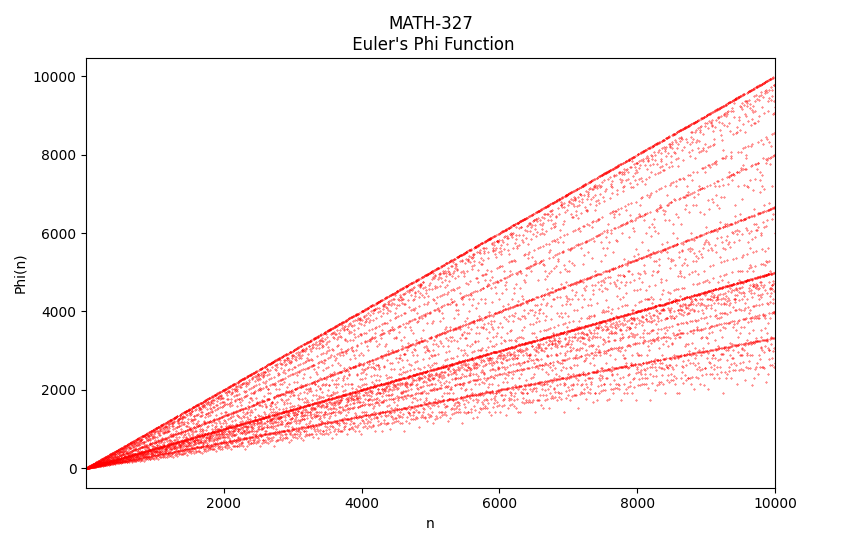
\includegraphics[scale=.4]{PHI.png}
  \caption{Euler's Phi function plotted up to 10,000}
  \label{fig:PhiPlot}
\end{figure}
\subsection{Conclusion}
The visual representations that arise from ideas in number theory are amazing to look at, and Euler's Phi function is no excuse. The power computers 
give us to generate these models is just another example of how technology can give us an insight into mathematical concepts.
\end{document}
